\documentclass[a4paper,10pt]{jsarticle}

% レイアウト
\setlength{\textwidth}{\fullwidth}
\setlength{\textheight}{39\baselineskip}
\addtolength{\textheight}{\topskip}
\setlength{\voffset}{-0.5in}
\setlength{\headsep}{0.3in}
\pagestyle{myheadings}

% パッケージ
\usepackage[dvipdfmx]{graphicx}
\usepackage{amsmath,amssymb,epsfig}
\usepackage{bm}
\usepackage{ascmac}
\usepackage{pifont}
\usepackage{multirow}
\usepackage{enumerate}
\usepackage{cases}
\usepackage{type1cm}
\usepackage{cancel}
\usepackage{url}
\usepackage[dvipdfmx]{color}
\usepackage{listings,jlisting}
% 大きな中括弧
\usepackage{cases}

% 定義
\DeclareMathOperator*{\argmin}{arg\,min}
\DeclareMathOperator*{\argmax}{arg\,max}
\def\vec#1{\mbox{\boldmath$#1$}}
\def\R{{\Bbb R}}

% カウンタの設定
\setcounter{section}{0}
\setcounter{subsection}{0}
\setcounter{subsubsection}{0}
\setcounter{equation}{0}

% キャプションの図をFigに変更
\renewcommand{\figurename}{Fig.}
\renewcommand{\tablename}{Tab.}

% 式番号を式(章番号.番号)に
% \makeatletter
% \renewcommand{\theequation}{\arabic{section}.\arabic{equation}}
% \@addtoreset{equation}{section}
% \makeatother

% プログラムに色をつける
\usepackage{color}

\definecolor{codegreen}{rgb}{0,0.6,0}
\definecolor{codegray}{rgb}{0.5,0.5,0.5}
\definecolor{codepurple}{rgb}{0.58,0,0.82}
\definecolor{backcolour}{rgb}{0.95,0.95,0.92}

\lstdefinestyle{mystyle}{
    backgroundcolor=\color{backcolour},
    commentstyle=\color{codegreen},
    keywordstyle=\color{magenta},
    numberstyle=\tiny\color{codegray},
    stringstyle=\color{codepurple},
    basicstyle=\footnotesize,
    breakatwhitespace=false,
    breaklines=true,
    captionpos=b,
    keepspaces=true,
    numbers=left,
    numbersep=5pt,
    showspaces=false,
    showstringspaces=false,
    showtabs=false,
    tabsize=2
}

\lstset{style=mystyle}

% 表紙
\title{知能システム学特論レポート}
\author{
(DL2班)Caffe on Ubuntu\\
}
\date{2015年\ 7月\ 21日}

% ドキュメントの開始
\begin{document}
\maketitle
\section{報告者}
\begin{list}{}{}
 \item 15344203\hspace{0.5cm} 有田 裕太
 \item 15344206\hspace{0.5cm} 緒形 裕太
 \item 15344209\hspace{0.5cm} 株丹 亮
 \item 12104125\hspace{0.5cm} 宮本 和
\end{list}

\section{進行状況}

\begin{itemize}
\item 畳み込みネットワークと正規化層の理論について
\item 独自の訓練データにより作成した識別器を用いた識別結果
\end{itemize}

\section{理論研究}

%%%%%% ogata %%%%%%
\subsection{誤差関数}
本班のcaffeを用いた画像分類では,第4回レポートで記したような多クラス分
類を行っており,出力関数はソフトマックス関数である.多クラス分類ではネッ
トワークが実現する関数を各クラスの事後確率のモデルであると見なし,そのモ
デルのもとで訓練データに対するネットワークパラメータの尤度を評価し,これ
を最大化する.いま訓練データとして,入力${\bf x}$とその正解クラスの組$C_k$が与え
られたとする.このときの目標出力の
2値の値を$K$個並べたベクトル${\bf
d}_n$によって表現すると,事後分布は次式のようになる.

\begin{equation}
 p({\bf d}|{\bf x}) = \prod_{k=1}^{K}p(C_k|{\bf x})^{d_k}
\end{equation}

これより,訓練データ${({\bf x}_n|{\bf d}_n)}(n=1,...,N)$に対する{\bf w}
の尤度は

\begin{equation}
 L({\bf w})=\prod_{n=1}^{N}p({\bf x}_n|{\bf x}_n;{\bf
	w})=\prod_{n=1}^{N}\prod_{k=1}^{K}p(C_k|{\bf
	x})^{d_{nk}}=\prod_{n=1}^{N}\prod_{k=1}^{K}(y_k({\bf x};{\bf w}))^{d_{nk}}
\end{equation}

と導ける.この尤度の対数とって符号を反転した次の式を誤差関数として用いる.
この関数は交差エントロピー(cross entropy)と呼ばれる.
\begin{eqnarray}
 E({\bf w})=-\sum^{N}_{n=1}\sum^{N}_{k=1}d_{nk}\log
	y_{k}(\vec{x}_{n};{\bf w})
\end{eqnarray}


\section{プログラミング}
\subsection{Pythonを用いたキャラクター識別用プログラムの作成}
前回までで独自のデータセットを用意して学習を行い,モデルを作成した.
Caffeでは.caffemodelという形式で保存され,これとCNNがどのように構成されているのかを表す.prototxtファイルを用いてキャラクター識別用プログラムを作成した.
これらを扱うためのCaffeが提供しているAPIと,画像を読み込んだり入力した画像に識別結果を書き込むためにOpenCVを用いた.

まず.caffemodelと.prototxtを読み込む部分のプログラムを示す.mean\_arrayは平均画像等が格納されているリストである.
raw\_scaleは読み込まれた入力画像をどのスケールにするかを指定する.

\begin{lstlisting}[basicstyle=\ttfamily\footnotesize, language=Python, frame=single, firstnumber=1, numbers=left, breaklines=true]
classifier = caffe.Classifier(
        'cifar10_full.prototxt',
        'cifar10_full_150717_iter_60000.caffemodel',
        mean=mean_array,
        raw_scale=255)
\end{lstlisting}

そして,入力画像からOpenCVで実装されているHaar-like特徴量から人の顔を抽出し,これをCaffeの識別器にかける.この部分のプログラムを示す.

\begin{lstlisting}[basicstyle=\ttfamily\footnotesize, language=Python, frame=single, firstnumber=1, numbers=left, breaklines=true]
predictions = classifier.predict([image], oversample=False)
pred = np.argmax(predictions)
\end{lstlisting}

classifier.predict()で抽出された顔が各ラベルの人の顔である確率がリターンされる.
そしてnumpyの関数を用いてnp.argmax()によって確率がリストとして代入されたpredictionsから最も高い確率のラベルを取得する.
この値と関連付けられたキャラクター名と確率の値をOpenCVのAPIを用いて入力画像に書き込む.
これをHaar-like特徴量から取得された顔の数だけ繰り返す.

\subsection{識別に用意した画像}
作成した識別器の性能を確認するために用意した画像をFig.\ref{224542_17Jul15}とFig.\ref{224550_17Jul15}に示す.Fig.\ref{224542_17Jul15}は学習したキャラクターしか含まれていないが,Fig.\ref{224550_17Jul15}では学習していないキャラクターしか含まれていない.従って,Fig.\ref{224542_17Jul15}ではキャラクター名それぞれに適切な名前が推定され,Fig.\ref{224550_17Jul15}では全て``etc''と推定されることが望ましい.

\begin{figure}[p]
 \centering
 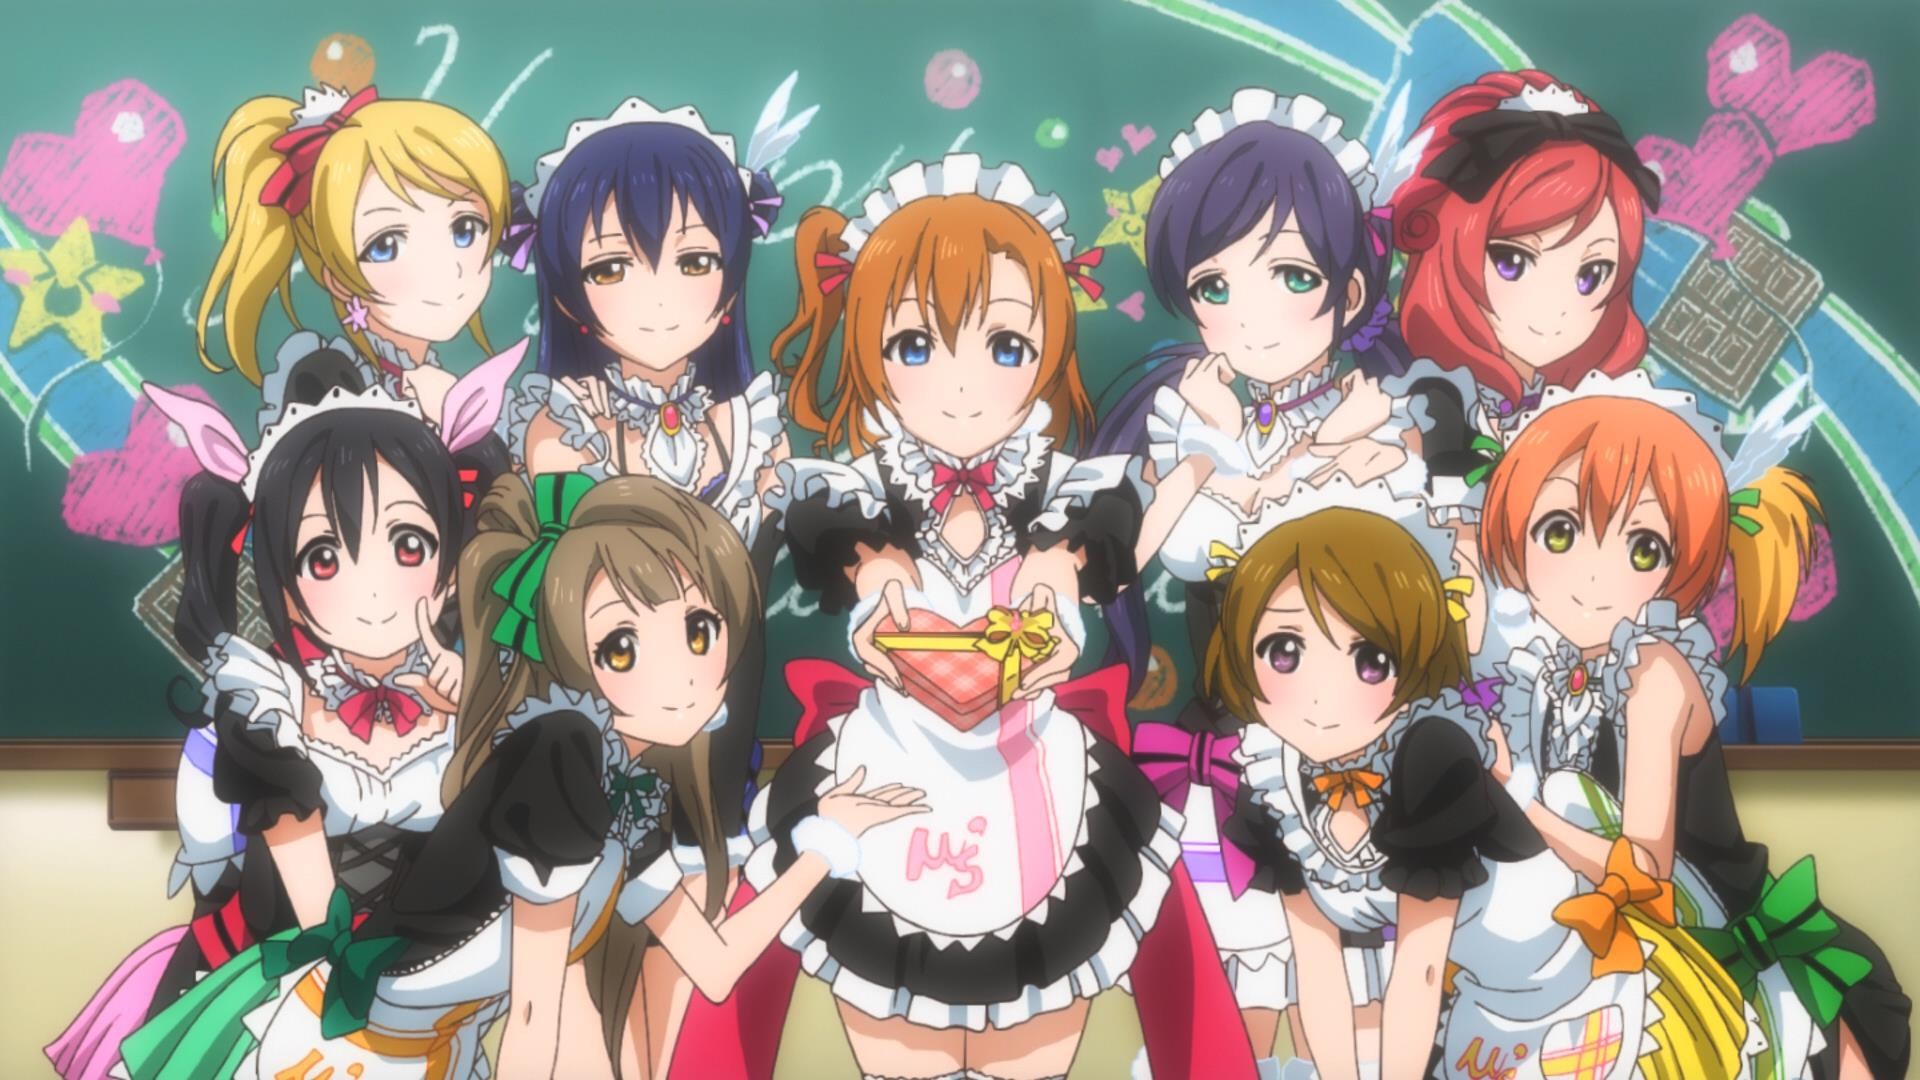
\includegraphics[width=140mm, bb = 0 0 1920 1080]{fig/jpg/lovelive.jpg}
 \caption{学習したキャラクターのみが含まれる画像 }
 \label{224542_17Jul15}
\end{figure}
\begin{figure}[bt]
 \centering
 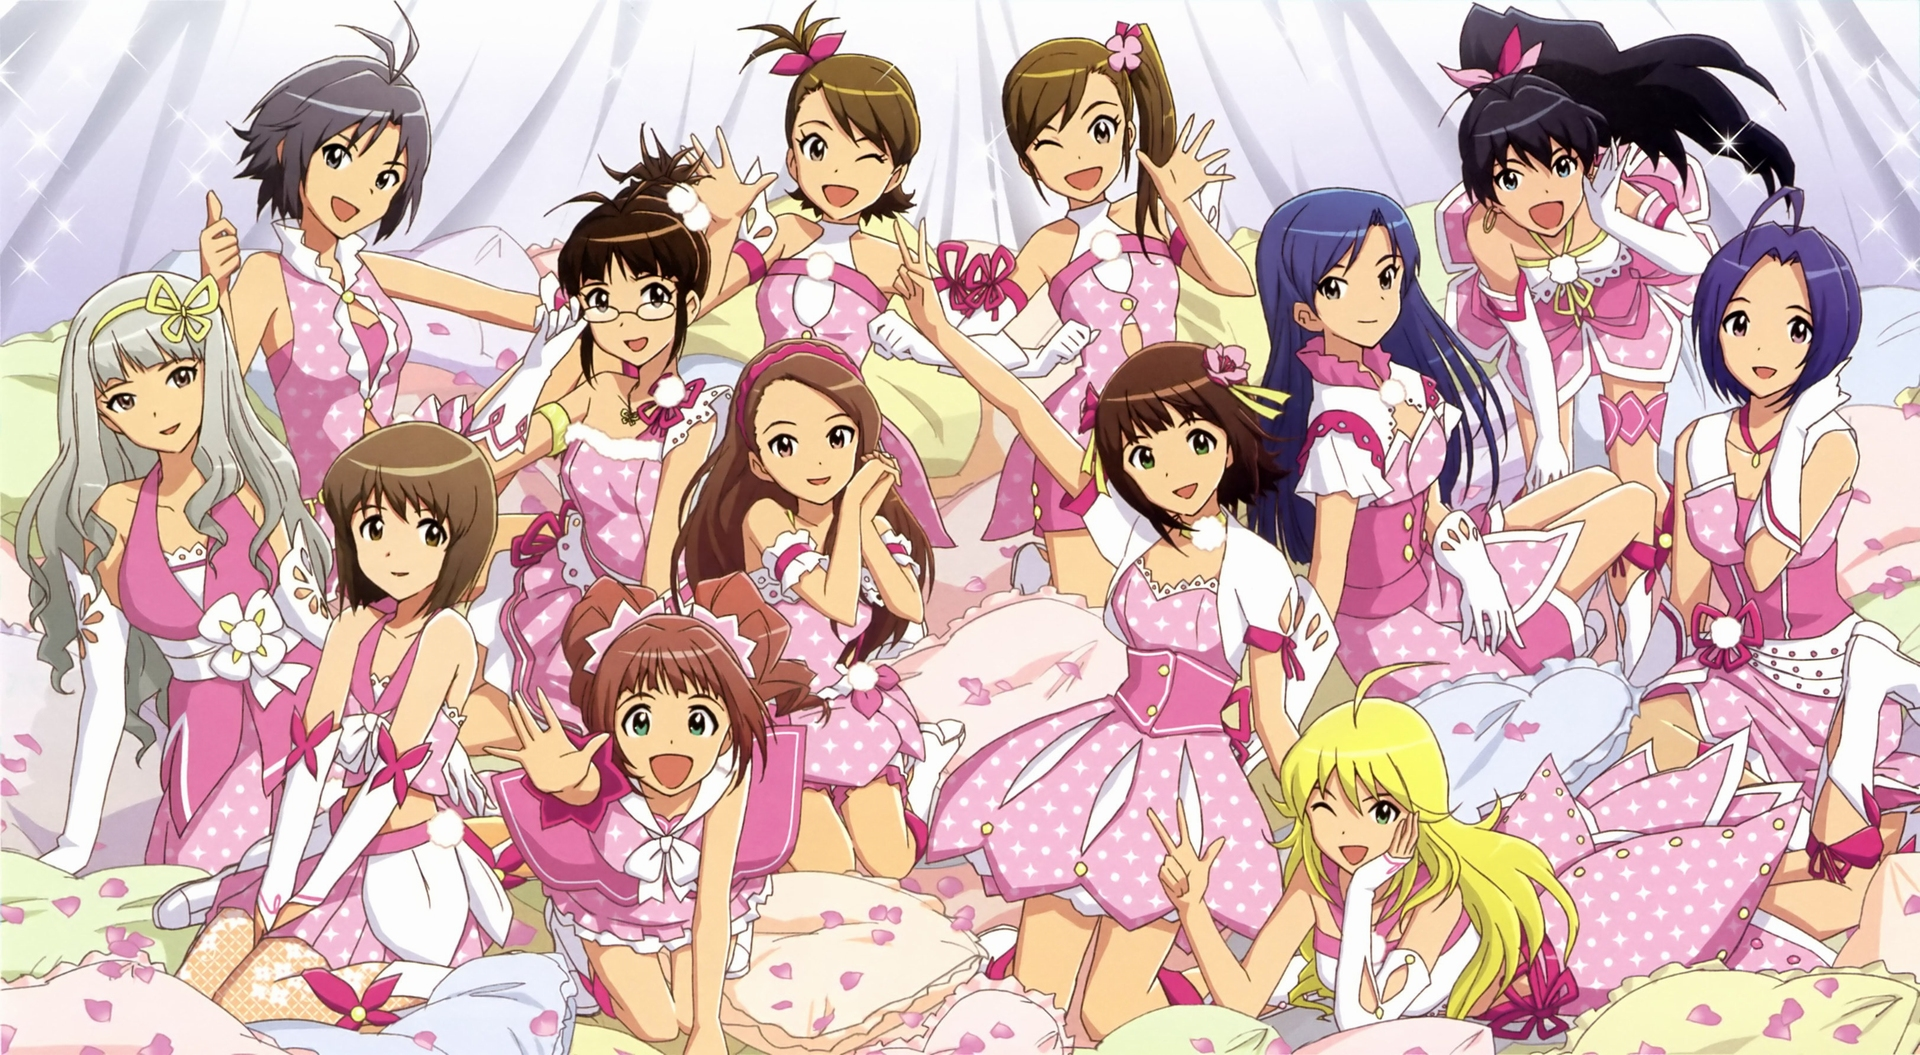
\includegraphics[width=140mm]{fig/jpg/idolmaster.jpg}
 \caption{学習したキャラクターが含まれていない画像 }
 \label{224550_17Jul15}
\end{figure}

\subsection{識別結果}
Fig.\ref{224542_17Jul15}とFig.\ref{224550_17Jul15}を識別した結果をそれぞれFig.\ref{224817_17Jul15}とFig.\ref{224823_17Jul15}に示す.Fig.\ref{224817_17Jul15}ではキャラクター名が全て適切に推定された.しかし,Fig.\ref{224823_17Jul15}では全て``etc''とならなければならないが一部のキャラクターで誤認識が発生した.誤認識が起こったキャラクターとそのラベルのキャラクターを比較すると髪の色が似ているなどの特徴があることが分かった.
\begin{figure}[bt]
 \centering
 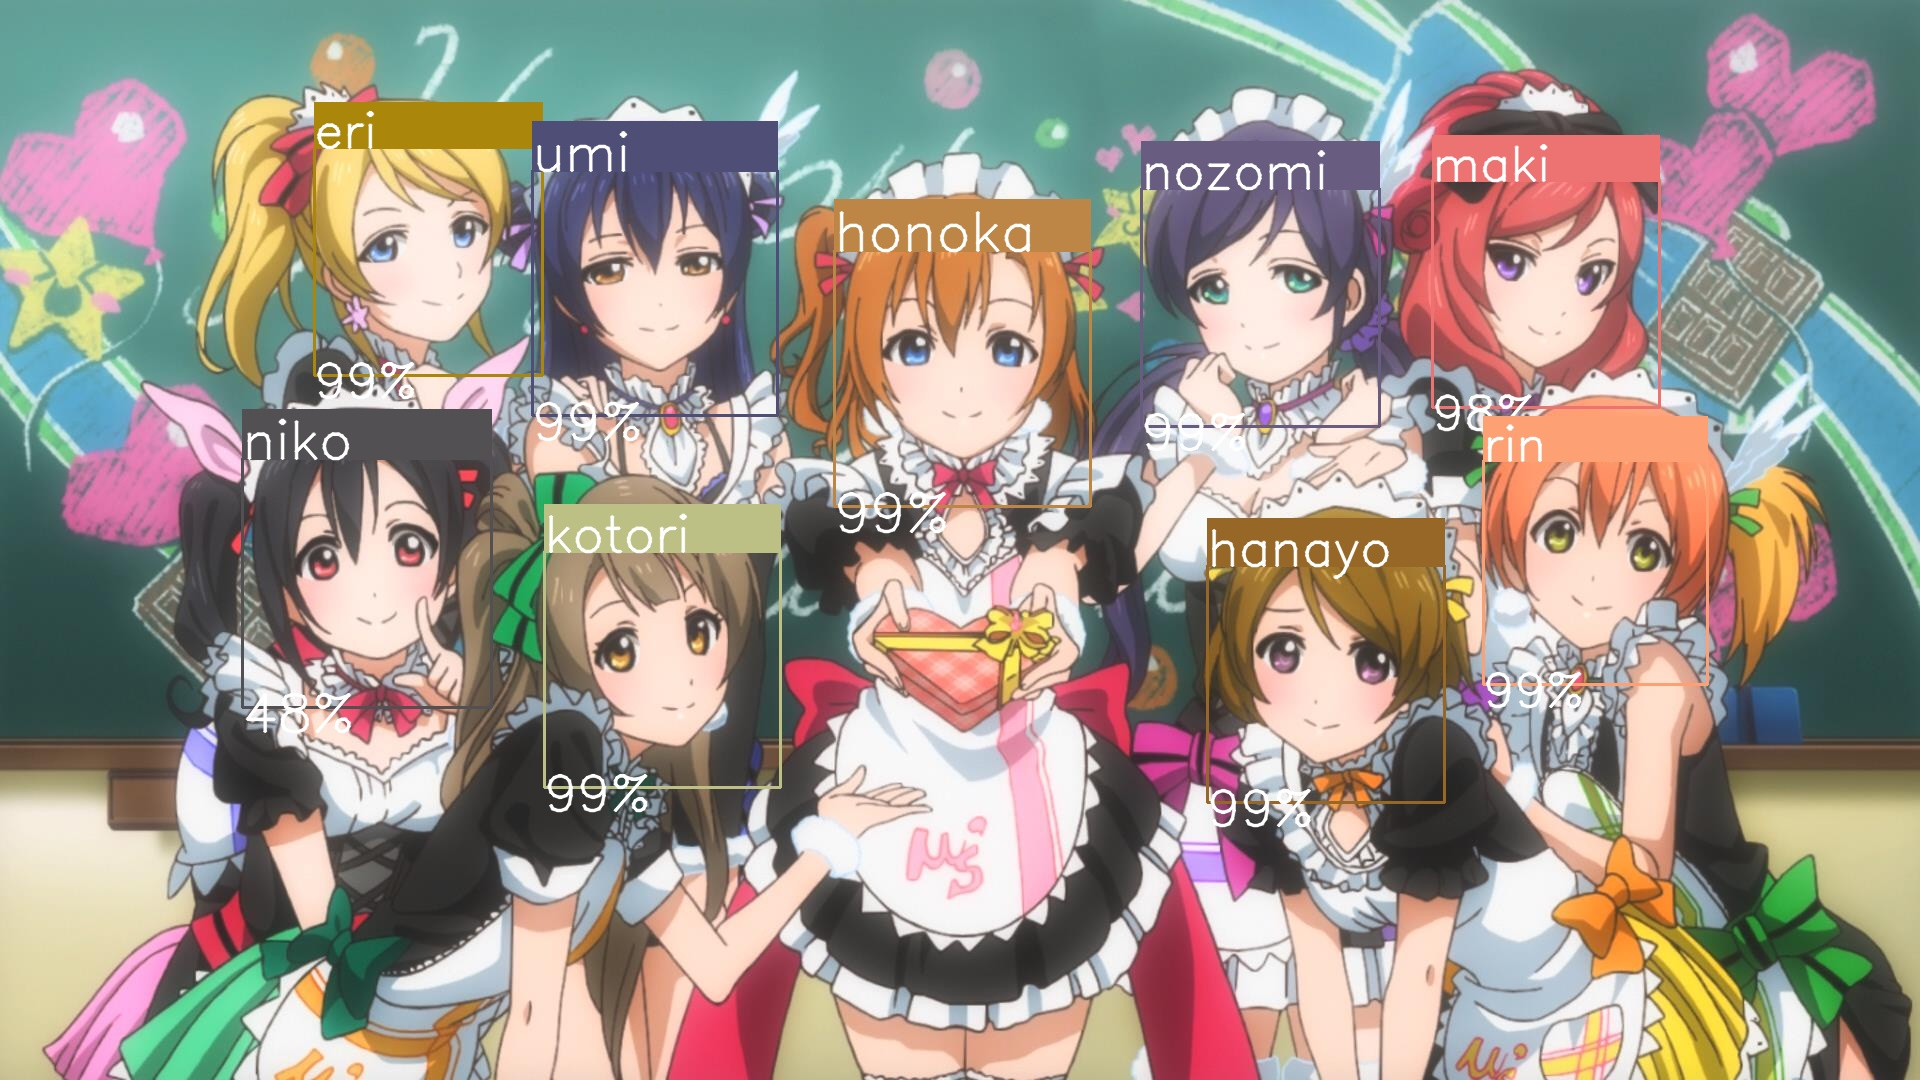
\includegraphics[width=140mm]{fig/jpg/result_lovelive.jpg}
 \caption{Fig.\ref{224542_17Jul15}の認識結果 }
 \label{224817_17Jul15}
\end{figure}
\begin{figure}[bt]
 \centering
 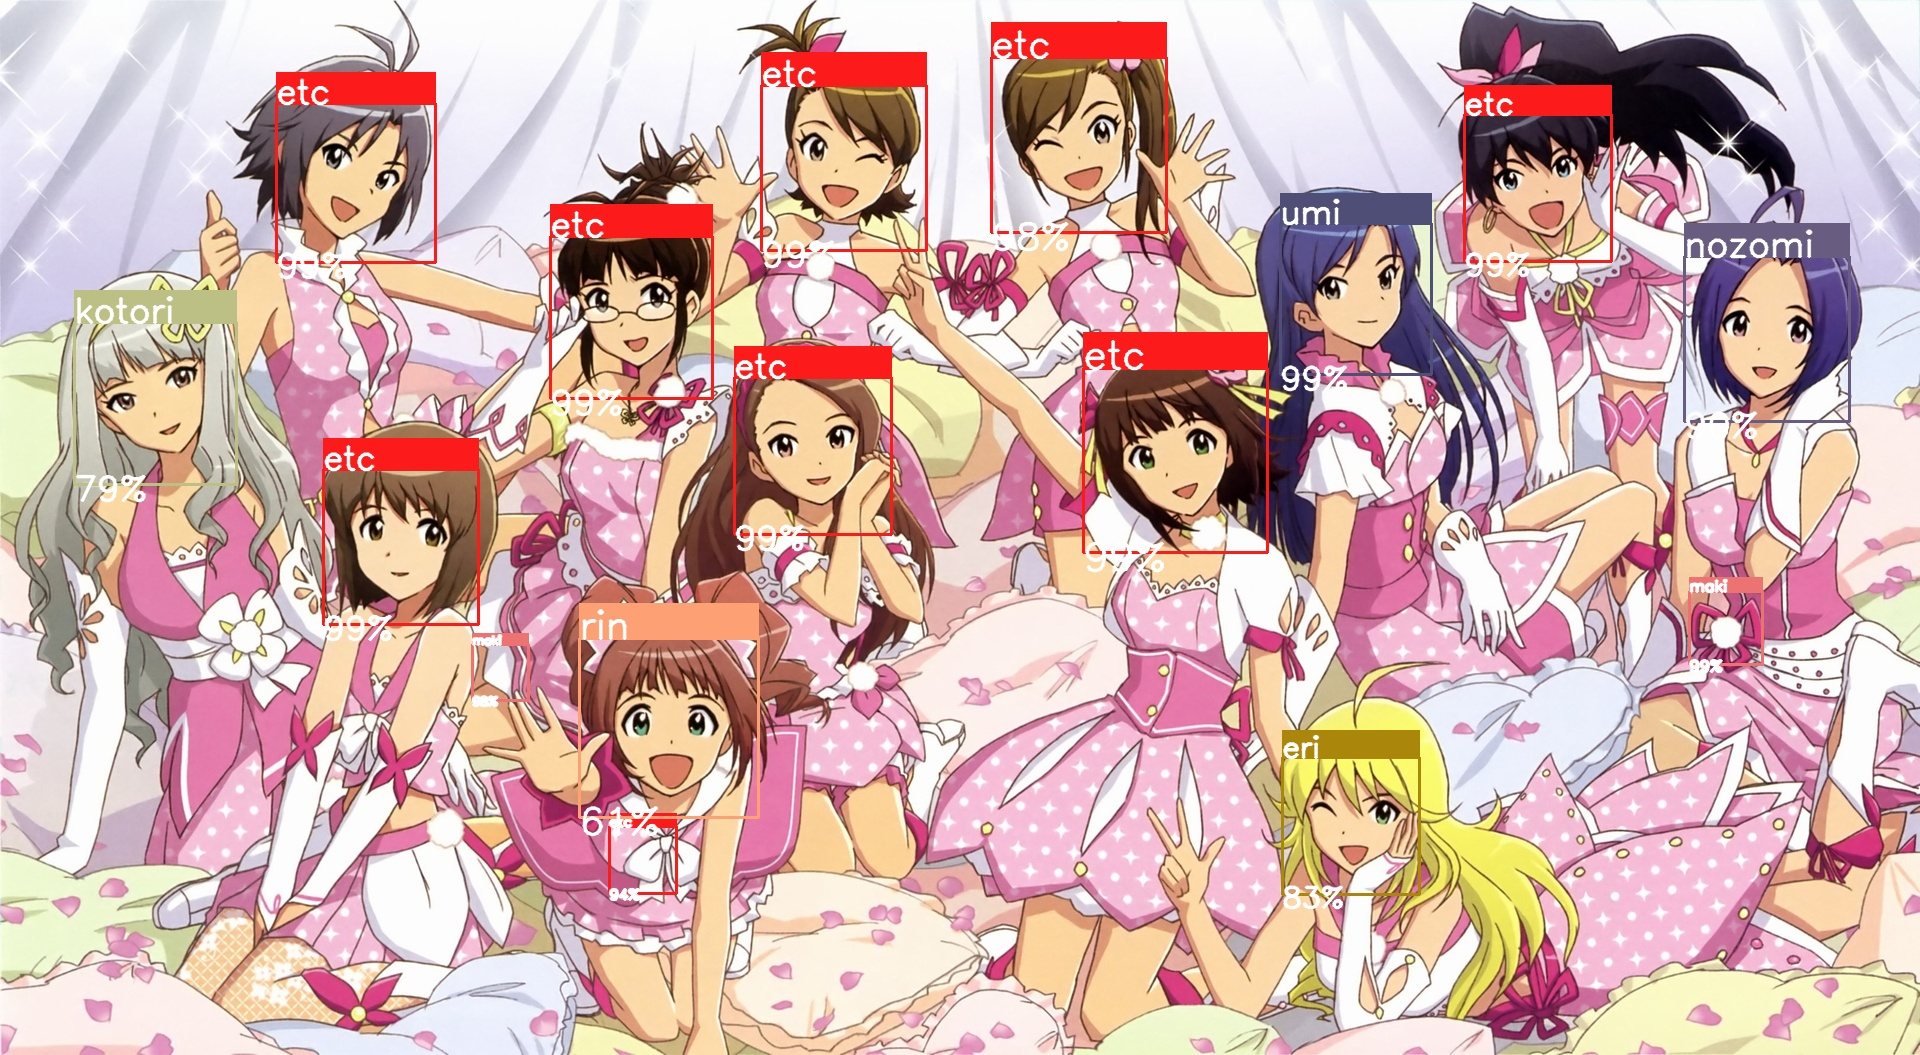
\includegraphics[width=140mm]{fig/jpg/result_idolmaster.jpg}
 \caption{Fig.\ref{224550_17Jul15}の認識結果 }
 \label{224823_17Jul15}
\end{figure}



\section{今後の課題}
\begin{itemize}
 \item 理論研究を進める.
 \item 作成した識別器でどのような特徴量が利用されているのかを調査する.
\end{itemize}

\end{document}